\documentclass[12pt, a4paper]{article}

\usepackage[margin=2.5cm]{geometry}
\usepackage{fontenc}
\usepackage{inputenc}
\usepackage{lmodern}
\usepackage{titlesec}
\usepackage{titling}
\usepackage{enumitem}
\usepackage{hyperref}
\usepackage{xcolor}
\usepackage{listings}
\usepackage{tabularx}
\usepackage{booktabs}
\usepackage{array}
\usepackage{fancyhdr}
\usepackage{parskip}
\usepackage{mdframed}
\usepackage{graphicx}
\usepackage{amsmath}
\usepackage{microtype}
\usepackage{tcolorbox}
\usepackage{tikz}
\usetikzlibrary{shapes.geometric, arrows.meta, positioning, fit, backgrounds}

% ── Colors ────────────────────────────────────────────────────────────────────
\definecolor{primary}{HTML}{5B21B6}
\definecolor{accent}{HTML}{2563EB}
\definecolor{codebg}{HTML}{F3F4F6}
\definecolor{codeframe}{HTML}{D1D5DB}
\definecolor{tableheadbg}{HTML}{EDE9FE}
\definecolor{notebg}{HTML}{FEF3C7}
\definecolor{noteframe}{HTML}{D97706}
\definecolor{bugbg}{HTML}{FEE2E2}
\definecolor{bugframe}{HTML}{DC2626}

% ── Hyperref ──────────────────────────────────────────────────────────────────
\hypersetup{
    colorlinks=true,
    linkcolor=primary,
    urlcolor=accent,
    citecolor=primary,
    pdfauthor={Pratik Suryavanshi},
    pdftitle={AI Placement Intelligence Agent — Technical Deep Dive},
}

% ── Listings (code) ───────────────────────────────────────────────────────────
\lstset{
    backgroundcolor=\color{codebg},
    frame=single,
    rulecolor=\color{codeframe},
    basicstyle=\ttfamily\small,
    breaklines=true,
    breakatwhitespace=true,
    showstringspaces=false,
    tabsize=4,
    xleftmargin=6pt,
    xrightmargin=6pt,
    captionpos=b,
    numbers=left,
    numberstyle=\tiny\color{gray},
    numbersep=6pt,
}

\lstdefinelanguage{pseudocode}{
    morekeywords={IF, ELSE, FOR, WHILE, RETURN, AND, OR, NOT, FUNCTION, END},
    sensitive=false,
    morecomment=[l]{//},
    morestring=[b]",
}

% ── Section styling ───────────────────────────────────────────────────────────
\titleformat{\section}{\Large\bfseries\color{primary}}{}{0em}{}[\titlerule]
\titleformat{\subsection}{\large\bfseries\color{accent}}{}{0em}{}
\titleformat{\subsubsection}{\normalsize\bfseries}{}{0em}{}

% ── Custom boxes ──────────────────────────────────────────────────────────────
\tcbuselibrary{skins, breakable}

\newtcolorbox{notebox}{
    colback=notebg, colframe=noteframe,
    boxrule=0.8pt, arc=4pt,
    left=6pt, right=6pt, top=4pt, bottom=4pt,
    fonttitle=\bfseries, title={Note},
}

\newtcolorbox{bugbox}{
    colback=bugbg, colframe=bugframe,
    boxrule=0.8pt, arc=4pt,
    left=6pt, right=6pt, top=4pt, bottom=4pt,
    fonttitle=\bfseries, title={Bug Fixed},
}

\newtcolorbox{interviewbox}{
    colback=tableheadbg, colframe=primary,
    boxrule=0.8pt, arc=4pt,
    left=6pt, right=6pt, top=4pt, bottom=4pt,
    fonttitle=\bfseries\color{white}, coltitle=white,
    attach boxed title to top left={yshift=-2mm, xshift=4mm},
    boxed title style={colback=primary, arc=3pt},
    title={Interview Q\&A},
    breakable,
}

% ── Header/Footer ─────────────────────────────────────────────────────────────
\pagestyle{fancy}
\fancyhf{}
\rhead{\small\textcolor{gray}{AI Placement Intelligence Agent}}
\lhead{\small\textcolor{gray}{Pratik Suryavanshi · 2023EE10264 · IIT Delhi}}
\rfoot{\small\thepage}
\renewcommand{\headrulewidth}{0.4pt}

% ── Title ─────────────────────────────────────────────────────────────────────
\title{
    \vspace{-1cm}
    {\Large\textbf{\textcolor{primary}{AI Placement Intelligence Agent}}}\\[0.3em]
    {\normalsize Technical Deep Dive --- Interview Preparation Guide}
}
\author{
    \textbf{Pratik Suryavanshi}\\
    2023EE10264 · B.Tech Electrical Engineering\\
    Indian Institute of Technology, Delhi\\
    \href{mailto:ee1230264@iitd.ac.in}{ee1230264@iitd.ac.in}
}
\date{June 2026}

% ══════════════════════════════════════════════════════════════════════════════
\begin{document}
% ══════════════════════════════════════════════════════════════════════════════

\maketitle
\thispagestyle{fancy}

\begin{abstract}
This document provides a thorough technical explanation of the \textbf{AI Placement Intelligence Agent} --- a fully local, privacy-first AI system built for IIT Delhi placement season. The system ingests PDF/DOCX job descriptions, extracts structured metadata, indexes them with vector embeddings, and exposes a conversational AI interface for intelligent querying. No internet connection or cloud API is required at inference time.
\end{abstract}

\tableofcontents
\newpage

% ══════════════════════════════════════════════════════════════════════════════
\section{Project Overview}
% ══════════════════════════════════════════════════════════════════════════════

The AI Placement Intelligence Agent solves a concrete problem at IIT Delhi: during placement season, students receive dozens of Job Description (JD) PDFs and must manually sift through them to find roles they are eligible for and interested in. This system automates that process.

\subsection{Core Capabilities}

\begin{itemize}[leftmargin=*, noitemsep]
    \item \textbf{Auto-ingestion} --- Drop a PDF into \texttt{jd\_files/}; the system discovers, parses, and indexes it automatically within seconds.
    \item \textbf{Semantic search} --- Ask ``Which companies need Python and offer above 15 LPA?'' and get cited answers.
    \item \textbf{Comparison} --- ``Compare Samsung vs Purplle'' builds a structured matrix.
    \item \textbf{Eligibility filtering} --- ``Recommend roles for a CSE student with 8.2 CGPA'' applies hard SQL filters before neural search.
    \item \textbf{Analytics} --- ``What is the average stipend across all internships?'' queries SQLite aggregations.
    \item \textbf{Conversation memory} --- Multi-turn: ``What about their deadline?'' resolves correctly from prior context.
    \item \textbf{File upload} --- Upload a PDF directly from the chat UI; duplicate detection prevents re-indexing.
\end{itemize}

\subsection{Privacy-First Design}

\begin{notebox}
All processing runs \textbf{100\% locally}. The LLM (llama3.2) runs via Ollama on the student's machine. No placement data is sent to any external server, cloud API, or third party. This is critical since IIT Delhi placement data is confidential.
\end{notebox}

% ══════════════════════════════════════════════════════════════════════════════
\section{System Architecture}
% ══════════════════════════════════════════════════════════════════════════════

\subsection{High-Level Flow}

\begin{center}
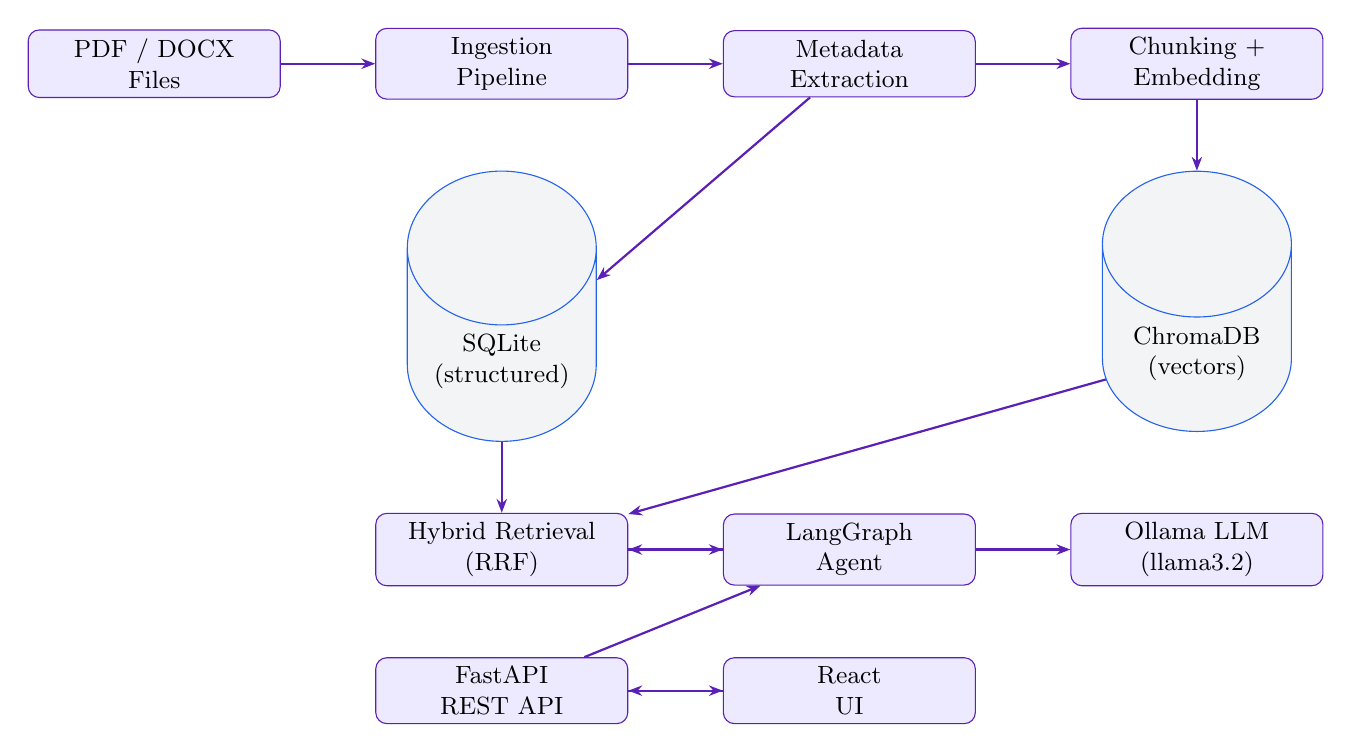
\begin{tikzpicture}[
    node distance=0.6cm and 1.2cm,
    box/.style={rectangle, rounded corners=4pt, draw=primary, fill=tableheadbg,
                minimum width=3.2cm, minimum height=0.8cm, align=center, font=\small},
    db/.style={cylinder, draw=accent, fill=codebg, shape border rotate=90,
               minimum width=2.4cm, minimum height=0.8cm, align=center, font=\small},
    arr/.style={-{Stealth[length=5pt]}, thick, color=primary}
]

\node[box] (pdf)    {PDF / DOCX\\Files};
\node[box, right=of pdf] (ingest) {Ingestion\\Pipeline};
\node[box, right=of ingest] (extract) {Metadata\\Extraction};
\node[box, right=of extract] (embed) {Chunking +\\Embedding};

\node[db, below=0.9cm of ingest] (sqlite) {SQLite\\(structured)};
\node[db, below=0.9cm of embed]  (chroma) {ChromaDB\\(vectors)};

\node[box, below=0.9cm of sqlite] (hybrid) {Hybrid Retrieval\\(RRF)};
\node[box, right=of hybrid] (agent) {LangGraph\\Agent};
\node[box, right=of agent]  (llm)   {Ollama LLM\\(llama3.2)};
\node[box, below=0.9cm of hybrid] (api)    {FastAPI\\REST API};
\node[box, right=of api]    (ui)    {React\\UI};

\draw[arr] (pdf) -- (ingest);
\draw[arr] (ingest) -- (extract);
\draw[arr] (extract) -- (embed);
\draw[arr] (extract) -- (sqlite);
\draw[arr] (embed) -- (chroma);
\draw[arr] (sqlite) -- (hybrid);
\draw[arr] (chroma) -- (hybrid);
\draw[arr] (hybrid) -- (agent);
\draw[arr] (agent) -- (llm);
\draw[arr] (agent) -- (hybrid);
\draw[arr] (api) -- (agent);
\draw[arr] (ui) -- (api);
\draw[arr] (api) -- (ui);

\end{tikzpicture}
\end{center}

\subsection{Component Responsibilities}

\begin{tabularx}{\textwidth}{>{\bfseries}lX}
\toprule
Component & Responsibility \\
\midrule
Watchdog & OS-level filesystem events; detects new files instantly without polling \\
PyMuPDF + Tesseract & Text extraction from digital and scanned PDFs \\
Rule / NLP / LLM Extractor & 3-stage cascade for structured metadata extraction \\
BGE-small-en-v1.5 & 384-dim sentence embeddings; asymmetric retrieval model \\
SQLite + SQLAlchemy & Structured storage: company, CTC, CGPA, skills, branches, locations \\
ChromaDB & HNSW vector index; cosine similarity search over chunk embeddings \\
Hybrid Retriever + RRF & Merges SQL and vector results by Reciprocal Rank Fusion \\
LangGraph & Stateful agent graph; 6 intent nodes; persistent conversation memory \\
OllamaClient & HTTP interface to local llama3.2 instance; lazy-loaded on first query \\
FastAPI & REST API; Pydantic validation; lifespan context manager for startup/shutdown \\
React + Vite & SPA frontend; glass-morphism design; drag-and-drop file upload \\
\bottomrule
\end{tabularx}

% ══════════════════════════════════════════════════════════════════════════════
\section{Ingestion Pipeline}
% ══════════════════════════════════════════════════════════════════════════════

\subsection{Stage 1 --- Discovery (Watchdog)}

The \texttt{DocumentDiscoveryModule} registers a \texttt{FileSystemEventHandler} with the \texttt{watchdog} library on the \texttt{jd\_files/} directory. When a new file appears (via OS inotify / FSEvents / ReadDirectoryChangesW), an event is pushed into a thread-safe \texttt{queue.Queue}. A separate indexing worker thread consumes from this queue.

This is \textbf{event-driven}, not polling --- the system reacts in under 100ms of a file appearing.

\subsection{Stage 2 --- Deduplication (SHA-256)}

Before any processing, the file's content is hashed using SHA-256. The hash is checked against the \texttt{documents.content\_hash} column in SQLite (indexed). Two deduplication checks:

\begin{enumerate}[noitemsep]
    \item \textbf{By filename} --- same filename already in database → skip
    \item \textbf{By content hash} --- same bytes with different filename → skip
\end{enumerate}

This prevents re-processing the same JD uploaded multiple times or renamed.

\subsection{Stage 3 --- Text Extraction}

\begin{tabularx}{\textwidth}{lX}
\toprule
\textbf{PDF type} & \textbf{Method} \\
\midrule
Digital (text-layer) & PyMuPDF reads text directly --- fast (\textasciitilde 50ms/page) \\
Scanned (image-only) & PyMuPDF renders each page as a PNG → Tesseract OCR reads it (\textasciitilde 3--5s/page) \\
DOCX & python-docx extracts paragraphs and tables \\
\bottomrule
\end{tabularx}

IIT Delhi JD forms are commonly scanned submissions, making Tesseract OCR a necessity rather than a fallback.

\subsection{Stage 4 --- Metadata Extraction (3-Stage Cascade)}

\subsubsection{Stage 4a: Rule-Based Extractor}

Uses compiled regular expressions for structured numerical fields:

\begin{lstlisting}[language=Python, caption=Sample regex patterns]
# CGPA cutoff
re.compile(r'(?:minimum|min\.?)\s*cgpa\s*[:\-]?\s*([0-9]+(?:\.[0-9]+)?)', re.I)

# Monthly stipend (handles "75,000", "75K", "75000")
re.compile(r'stipend.*?(\d[\d,]*(?:\.\d+)?)\s*(?:k|thousand|lakh)?', re.I)

# Duration (1-12 months)
re.compile(r'\b(1[0-2]|[1-9])\s*months?\b', re.I)

# Job type (order: PPO first, then FTE, then internship)
# PPO must be checked before internship to avoid misclassification
\end{lstlisting}

\begin{bugbox}
\textbf{CGPA regex} originally used \texttt{[0-9]} which matched only single digits --- couldn't match 10.0. Fixed to \texttt{[0-9]+}.\\
\textbf{Job type order} was wrong: internship was checked before PPO. A PPO notice was being classified as ``internship''. Fixed by checking PPO first.
\end{bugbox}

\subsubsection{Stage 4b: NLP Extractor}

Keyword matching with word-boundary guards (\verb|\b|) against curated lists:

\begin{itemize}[noitemsep]
    \item \textbf{Skills}: Python, Golang, React, MongoDB, Kubernetes, \ldots (single-character entries like \texttt{"c"} and \texttt{"r"} were removed --- they matched random letters everywhere)
    \item \textbf{Locations}: Bangalore, Mumbai, Gurgaon, Remote, \ldots (with canonical mapping: bengaluru → Bangalore, gurugram → Gurgaon)
    \item \textbf{Branches}: CSE, ECE, EE, MnC, MT, PH, MA, ALL, \ldots
\end{itemize}

\subsubsection{Stage 4c: LLM Fallback}

When company name and role title cannot be extracted by rules or NLP, a single LLM call to llama3.2 extracts them. This is the \textbf{most expensive stage} (2--10 seconds) and is only triggered if the earlier stages fail.

\subsection{Stage 5 --- Semantic Chunking}

The full document text is split into overlapping chunks:

\begin{itemize}[noitemsep]
    \item \textbf{Chunk size}: 400 tokens (\textasciitilde 300 words)
    \item \textbf{Overlap}: 60 tokens (prevents information loss at boundaries)
    \item \textbf{Section-aware}: If the document has headers (``Eligibility'', ``Stipend Details''), chunks align to section boundaries first
    \item \textbf{Fallback}: If no sections detected (common in OCR output), the plain text is chunked uniformly
\end{itemize}

\begin{bugbox}
When \texttt{doc.sections == []}, the chunker loop produced \textbf{zero chunks} --- the document was silently lost from vector search. Fixed by adding a \texttt{\_chunk\_plain\_text()} fallback called when no section-based chunks are produced.
\end{bugbox}

\subsection{Stage 6 --- Embedding}

The \texttt{BAAI/bge-small-en-v1.5} model (84MB, 384 dimensions) converts each chunk into a float vector. This model uses \textbf{asymmetric retrieval}:

\begin{itemize}[noitemsep]
    \item \textbf{Documents}: embedded as plain text
    \item \textbf{Queries}: prefixed with \texttt{"Represent this job description for retrieval: "}
\end{itemize}

\begin{bugbox}
The instruction prefix was being prepended to \textbf{document chunks} as well --- a violation of BGE's asymmetric design that degrades retrieval quality. Fixed by adding a separate \texttt{embed\_query()} method that applies the prefix only to query vectors.
\end{bugbox}

A separate \textbf{embedding cache} in SQLite stores computed embeddings keyed by content SHA-256. Re-indexing the same chunk (e.g., after a re-scan) skips the model call entirely.

% ══════════════════════════════════════════════════════════════════════════════
\section{Database Design}
% ══════════════════════════════════════════════════════════════════════════════

\subsection{SQLite Schema (structured data)}

The system uses two SQLite databases:

\subsubsection{metadata.db --- JD data}

\begin{center}
\begin{tikzpicture}[
    table/.style={rectangle, draw=accent, rounded corners=3pt, fill=codebg,
                  font=\ttfamily\footnotesize, align=left, inner sep=6pt},
    fk/.style={-{Stealth[length=4pt]}, dashed, color=gray}
]
\node[table] (doc) {
    \textbf{documents}\\
    \hline
    doc\_id (PK)\\
    file\_name\\
    content\_hash (UNIQUE)\\
    status [pending|indexed|failed]\\
    discovered\_at, indexed\_at
};

\node[table, right=1.5cm of doc] (meta) {
    \textbf{jd\_metadata}\\
    \hline
    metadata\_id (PK)\\
    doc\_id (FK)\\
    company\_name\\
    role\_title, job\_type\\
    package\_ctc, stipend\_monthly\\
    cgpa\_cutoff, deadline\\
    work\_mode, duration\_months
};

\node[table, below=0.7cm of doc] (skills) {
    \textbf{jd\_skills}\\
    \hline
    id (PK)\\
    doc\_id (FK)\\
    skill, skill\_normalized
};

\node[table, right=1.5cm of skills] (locs) {
    \textbf{jd\_locations}\\
    \hline
    id (PK)\\
    doc\_id (FK)\\
    location
};

\node[table, right=1.5cm of locs] (branches) {
    \textbf{jd\_branches}\\
    \hline
    id (PK)\\
    doc\_id (FK)\\
    branch\_code
};

\draw[fk] (meta.west) -- (doc.east);
\draw[fk] (skills.north) -- (doc.south);
\draw[fk] (locs) -- (skills.east);
\draw[fk] (branches) -- (locs.east);
\end{tikzpicture}
\end{center}

All child tables have \textbf{CASCADE DELETE} --- removing a document automatically removes all its skills, locations, branches, and metadata. This ensures no orphaned rows.

\textbf{SQLite pragmas applied at connection time:}
\begin{lstlisting}[language=SQL]
PRAGMA foreign_keys = ON;   -- enforce referential integrity
PRAGMA journal_mode = WAL;  -- concurrent reads don't block writes
\end{lstlisting}

WAL (Write-Ahead Log) mode is critical here because the background indexer thread writes while the FastAPI server reads --- without WAL, they would block each other.

\subsection{ChromaDB (vector data)}

\begin{itemize}[noitemsep]
    \item Collection name: \texttt{jd\_chunks}
    \item Distance metric: \textbf{cosine} (HNSW index)
    \item Each record: \texttt{chunk\_id}, \texttt{embedding[384]}, \texttt{document} (raw text), \texttt{metadata} (doc\_id, company\_name, job\_type, page\_number)
    \item Similarity score: \texttt{1.0 - distance/2.0} (cosine distance ∈ [0,2], similarity ∈ [0,1])
\end{itemize}

\subsection{checkpoints.db --- Conversation memory}

A separate SQLite file managed entirely by \textbf{LangGraph's SqliteSaver}. Stores the full agent state after every turn, keyed by \texttt{session\_id}. Enables multi-turn conversation without the application needing to manage state explicitly.

% ══════════════════════════════════════════════════════════════════════════════
\section{Hybrid Retrieval and RRF}
% ══════════════════════════════════════════════════════════════════════════════

\subsection{Why Two Systems?}

\begin{tabularx}{\textwidth}{lXX}
\toprule
 & \textbf{SQLite (BM25-style SQL)} & \textbf{ChromaDB (Vector)} \\
\midrule
Best at & Exact filters: \texttt{cgpa\_cutoff <= 7.5}, \texttt{job\_type = internship} & Semantic understanding: ``roles involving distributed systems'' \\
Fails at & Synonyms and meaning & Exact numeric comparisons \\
Speed & \textasciitilde 5ms & \textasciitilde 20--50ms \\
\bottomrule
\end{tabularx}

Neither alone is sufficient. A hybrid approach retrieves from both and merges.

\subsection{Reciprocal Rank Fusion (RRF)}

For each retrieved document:

\[
\text{RRF score} = \frac{1}{\text{rank}_{SQL} + k} + \frac{1}{\text{rank}_{vector} + k}, \quad k = 60
\]

The constant $k = 60$ prevents very low ranks (e.g., rank 1) from dominating the score. Documents that appear high in \textbf{both} systems rise to the top. Documents appearing in only one system are still included but score lower.

\subsection{Entity Extraction from Queries}

Before retrieval, \texttt{QueryEntityExtractor} parses the query text:

\begin{itemize}[noitemsep]
    \item \textbf{Company names}: matched against known companies from SQLite
    \item \textbf{Package}: regex patterns for ``15 LPA'', ``CTC above 20'', ``15 lakhs''
    \item \textbf{CGPA}: ``7.5 CGPA'', ``cgpa cutoff 8'', ``cgpa >= 6.5''
    \item \textbf{Job type}: intern, FTE, full-time
    \item \textbf{Skills}: against a curated list of 40+ technologies
    \item \textbf{Locations}: against Indian city names with canonical mapping
\end{itemize}

% ══════════════════════════════════════════════════════════════════════════════
\section{LangGraph Agent}
% ══════════════════════════════════════════════════════════════════════════════

\subsection{What is LangGraph?}

LangGraph is a framework for building \textbf{stateful, multi-step AI agent pipelines} as directed graphs. Each node is a Python function; edges define control flow. The shared state (\texttt{AgentState}) is a \texttt{TypedDict} passed between nodes.

\subsection{Agent State}

\begin{lstlisting}[language=Python]
class AgentState(TypedDict, total=False):
    query_text: str          # original user query
    resolved_query: str      # expanded query (after followup resolution)
    intent: str              # search | compare | recommend | analytics | summary | followup
    retrieved_chunks: List   # raw chunks from hybrid retrieval
    source_documents: List   # cited documents with metadata
    response_text: str       # LLM-generated answer
    structured_data: dict    # comparison matrix, analytics numbers
    user_profile: dict       # cgpa, branch, skills, preferred locations
    turn_history: List       # last 10 conversation turns
    final_response: dict     # packaged API response
\end{lstlisting}

\subsection{Graph Topology}

\begin{center}
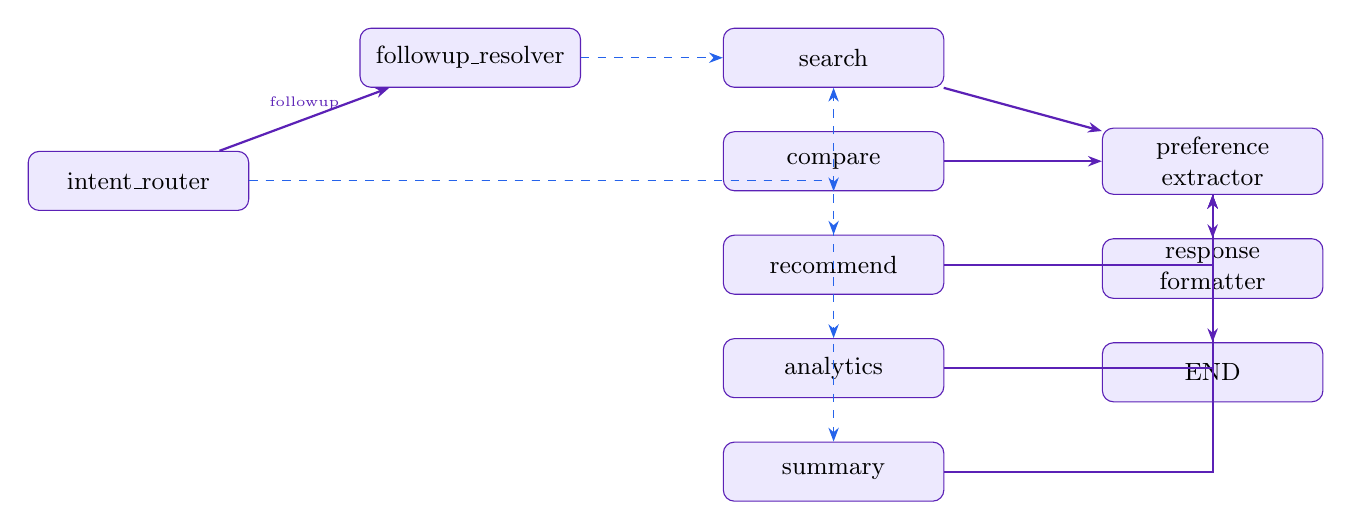
\begin{tikzpicture}[
    node distance=0.5cm and 1.8cm,
    n/.style={rectangle, rounded corners=4pt, draw=primary, fill=tableheadbg,
              minimum width=2.8cm, minimum height=0.75cm, align=center, font=\small},
    e/.style={-{Stealth[length=5pt]}, thick, color=primary},
    de/.style={-{Stealth[length=5pt]}, dashed, color=accent}
]
\node[n] (router)   {intent\_router};
\node[n, above right=0.8cm and 1.4cm of router] (follow) {followup\_resolver};
\node[n, right=1.8cm of follow] (search)  {search};
\node[n, below=0.55cm of search]  (compare) {compare};
\node[n, below=0.55cm of compare] (recommend) {recommend};
\node[n, below=0.55cm of recommend] (analytics) {analytics};
\node[n, below=0.55cm of analytics] (summary)  {summary};
\node[n, right=2cm of compare] (pref) {preference\\extractor};
\node[n, below=0.55cm of pref] (fmt)  {response\\formatter};
\node[n, below=0.55cm of fmt]  (end)  {END};

\draw[e] (router) -- node[above, font=\tiny]{followup} (follow);
\draw[de] (router) -| (search);
\draw[de] (router) -| (compare);
\draw[de] (router) -| (recommend);
\draw[de] (router) -| (analytics);
\draw[de] (router) -| (summary);
\draw[de] (follow) -- (search);
\draw[e] (search) -- (pref);
\draw[e] (compare) -- (pref);
\draw[e] (recommend) -| (pref);
\draw[e] (analytics) -| (pref);
\draw[e] (summary) -| (pref);
\draw[e] (pref) -- (fmt);
\draw[e] (fmt) -- (end);
\end{tikzpicture}
\end{center}

\subsection{Intent Detection}

\begin{tabularx}{\textwidth}{lX}
\toprule
\textbf{Intent} & \textbf{Trigger Keywords/Patterns} \\
\midrule
\texttt{compare}   & ``vs'', ``compare'', ``difference between'', ``better'' \\
\texttt{recommend} & ``recommend'', ``suggest'', ``best for me'', ``am I eligible'' \\
\texttt{analytics} & ``how many'', ``average'', ``trend'', ``statistics'' \\
\texttt{summary}   & ``summarize'', ``tell me about'', ``details of'' \\
\texttt{followup}  & ``this company'', ``that role'', ``previously mentioned'', ``same company'' \\
\texttt{search}    & Default (everything else) \\
\bottomrule
\end{tabularx}

\begin{bugbox}
Originally, words like \texttt{"it"}, \texttt{"them"}, \texttt{"that"} triggered followup intent. These appear in almost every English sentence, so nearly every first-turn query was misclassified as followup. Fixed by replacing single-word triggers with explicit phrase patterns using compiled regex.
\end{bugbox}

\subsection{Agent Node Descriptions}

\subsubsection{search\_node}
Runs the full hybrid retrieval pipeline and passes the assembled context to the LLM with a search-specific system prompt. Returns cited source documents.

\subsubsection{comparison\_node}
\begin{enumerate}[noitemsep]
    \item Extracts company names from the query
    \item Fetches their \texttt{JDMetadata} rows from SQLite
    \item Retrieves text chunks using \texttt{get\_chunks\_by\_doc\_id()} (not vector similarity --- chunks are fetched directly)
    \item Builds a structured comparison matrix
    \item Sends to LLM with a comparison-specific prompt
    \item \textbf{Post-hoc fact verification}: checks if the generated text contains the correct numerical values (CTC, CGPA) from SQLite; appends corrections if not
\end{enumerate}

\begin{bugbox}
Was using a \texttt{[0.0]*384} zero-vector for similarity search to retrieve chunks. A zero vector gives meaningless cosine similarity scores and retrieves random chunks. Fixed by adding \texttt{get\_chunks\_by\_doc\_id()} to ChromaDB which fetches stored chunks directly without any similarity computation.
\end{bugbox}

\subsubsection{recommendation\_node}
\begin{enumerate}[noitemsep]
    \item Reads \texttt{user\_profile} from state (CGPA, branch, skills)
    \item Queries SQLite with hard eligibility filters (e.g., \texttt{cgpa\_cutoff <= user\_cgpa})
    \item Runs vector search \textit{only within} the eligible document set using a ChromaDB \texttt{where} filter
    \item This prevents recommending ineligible roles even if they are semantically similar
\end{enumerate}

\subsubsection{preference\_extractor\_node}
Runs after \textit{every} agent node. Silently extracts any user preferences mentioned in the query (CGPA, skills, job type, location preferences) and updates the persistent \texttt{user\_profile} in state. So if a user asks ``show me Python roles for 8.0 CGPA'', future recommendations automatically apply those filters without the user repeating themselves.

\subsection{Conversation Memory}

LangGraph's \texttt{SqliteSaver} checkpointer persists the full \texttt{AgentState} to \texttt{data/checkpoints.db} after every node execution. On the next API request with the same \texttt{session\_id}, the graph loads the saved state and has access to:

\begin{itemize}[noitemsep]
    \item \texttt{turn\_history} (last 10 turns) --- which companies were discussed
    \item \texttt{user\_profile} --- preferences accumulated across turns
    \item \texttt{interacted\_doc\_ids} --- which JDs were referenced
\end{itemize}

% ══════════════════════════════════════════════════════════════════════════════
\section{Backend API}
% ══════════════════════════════════════════════════════════════════════════════

\subsection{FastAPI Design Choices}

\begin{itemize}[noitemsep]
    \item \textbf{Lifespan context manager} (\texttt{@asynccontextmanager}) handles startup (load models, connect DBs, start workers) and shutdown (stop workers, dispose SQLAlchemy engine) cleanly
    \item \textbf{Pydantic models} validate all request/response shapes at the boundary
    \item \textbf{CORS middleware} allows the React dev server (port 5173) to call the API (port 8000)
    \item \textbf{Application state} (\texttt{app.state}) holds shared singletons: \texttt{db\_manager}, \texttt{chroma\_manager}, \texttt{embedding\_pipeline}, \texttt{graph}
\end{itemize}

\subsection{Key Endpoints}

\begin{tabularx}{\textwidth}{llX}
\toprule
\textbf{Method} & \textbf{Path} & \textbf{Purpose} \\
\midrule
GET  & \texttt{/api/index/health} & System health check (SQLite, ChromaDB, Ollama status) \\
POST & \texttt{/api/query}        & Main chat endpoint; invokes LangGraph agent graph \\
GET  & \texttt{/api/documents}   & All indexed JDs with nested metadata for the Browse page \\
POST & \texttt{/api/upload}      & Upload a new JD PDF/DOCX; deduplicates by name + SHA-256 hash \\
GET  & \texttt{/api/analytics/summary} & Aggregated stats for the Analytics dashboard \\
PUT  & \texttt{/api/profile/\{session\_id\}} & Update user profile (CGPA, branch, skills) \\
\bottomrule
\end{tabularx}

\subsection{Caching Layer}

\begin{itemize}[noitemsep]
    \item \textbf{Query cache} (\texttt{TTL = 5 min, max 100 entries}): identical query + session ID combos return instantly
    \item \textbf{Analytics cache} (\texttt{TTL = 24h, max 10 entries}): expensive aggregation queries are cached; invalidated when a new document is indexed
\end{itemize}

% ══════════════════════════════════════════════════════════════════════════════
\section{Frontend}
% ══════════════════════════════════════════════════════════════════════════════

\subsection{Tech Stack}

\begin{tabularx}{\textwidth}{lX}
\toprule
\textbf{Tool} & \textbf{Role} \\
\midrule
React 18 + Vite    & Component model; HMR for fast development \\
Tailwind CSS v3    & Utility-first styling; no custom CSS files \\
Framer Motion      & Declarative animations (page transitions, bubble entry, drag overlay) \\
Lucide React       & Icon set \\
react-markdown     & Renders LLM markdown output (bold, lists, code blocks) in chat \\
\bottomrule
\end{tabularx}

\subsection{Pages}

\begin{description}[leftmargin=2cm, style=nextline]
    \item[Chat Page] Multi-turn conversation with the AI; file upload (click or drag-and-drop); markdown-rendered responses; session ID stored in \texttt{sessionStorage}
    \item[Browse JDs] Split panel: searchable list + detail panel with skills chips, branches, status; ``Scan'' button triggers re-indexing
    \item[Analytics] Animated skill frequency bars; job type breakdown; recent documents list
    \item[Profile] CGPA input; branch selector; skills and location chip editors; saved via \texttt{PUT /api/profile/\{session\_id\}}
\end{description}

\subsection{File Upload Flow}

\begin{enumerate}[noitemsep]
    \item User clicks 📎 or drops a file onto the chat
    \item \texttt{FormData} sent to \texttt{POST /api/upload}
    \item Backend checks by filename → then by SHA-256 hash
    \item If new: saved to \texttt{jd\_files/}, \texttt{force\_rescan()} called, analytics cache cleared
    \item If existing: returns company/role info for the existing record
    \item Banner shown in chat: green (queued) / amber (already exists) / red (error)
\end{enumerate}

% ══════════════════════════════════════════════════════════════════════════════
\section{RAM Management}
% ══════════════════════════════════════════════════════════════════════════════

The system is designed to run on an 8GB laptop alongside a browser and IDE.

\begin{tabularx}{\textwidth}{lll}
\toprule
\textbf{Component} & \textbf{RAM} & \textbf{When loaded} \\
\midrule
BGE-small-en-v1.5 embedding model & 84 MB  & Startup (always) \\
ChromaDB + SQLite                 & 20 MB  & Startup (always) \\
FastAPI + Python runtime          & 50 MB  & Startup (always) \\
React Vite dev server             & 65 MB  & Startup (always) \\
\textbf{llama3.2:latest (Ollama)} & \textbf{2.0 GB} & \textbf{First chat query only} \\
\midrule
\textbf{Total peak}               & \textbf{\textasciitilde 6 GB} & (during chat) \\
\bottomrule
\end{tabularx}

\textbf{Key choices for RAM efficiency:}
\begin{itemize}[noitemsep]
    \item \texttt{BAAI/bge-small-en-v1.5} chosen over larger models (bge-large: 1.3GB) --- 384-dim vs 1024-dim, similar accuracy for JD retrieval
    \item \texttt{llama3.2:latest} (2GB) chosen over larger models (llama3.1:8b: 4.7GB) for fitting within 8GB budget
    \item LLM is \textbf{lazy-loaded} --- Ollama only loads it into RAM on the first request
    \item Embedding cache in SQLite prevents re-computing vectors on re-index
\end{itemize}

% ══════════════════════════════════════════════════════════════════════════════
\section{Common Interview Questions}
% ══════════════════════════════════════════════════════════════════════════════

\begin{interviewbox}

\textbf{Q: Why did you choose a local LLM instead of OpenAI?}\\
Privacy. IIT Delhi placement data is confidential. Running llama3.2 via Ollama means no data leaves the machine. Also zero recurring API cost.\\[6pt]

\textbf{Q: Why SQLite instead of PostgreSQL?}\\
SQLite with WAL mode is sufficient for a single-node system with under 10,000 documents. No server to manage, file-based, ships with Python. WAL mode enables concurrent reads and writes without blocking.\\[6pt]

\textbf{Q: What is RRF and why use it?}\\
Reciprocal Rank Fusion merges ranked lists from different retrieval systems: $\text{score} = \sum_i \frac{1}{k + \text{rank}_i}$ where $k=60$. It is robust because it uses rank positions rather than raw scores, which may be on incomparable scales across systems.\\[6pt]

\textbf{Q: What is asymmetric retrieval?}\\
In asymmetric retrieval, the query and the document are embedded differently. BGE prepends an instruction to the query (``Represent this job description for retrieval: ''), which shifts its embedding toward the document space. Applying the same instruction to documents degrades retrieval --- this was a bug we caught and fixed.\\[6pt]

\textbf{Q: How does the system handle scanned PDFs?}\\
PyMuPDF detects that there is no text layer and renders each page as a PNG image. Tesseract OCR reads the image and returns text. IIT Delhi's JD forms are typically scanned student submissions.\\[6pt]

\textbf{Q: What happens if the LLM hallucinates a number?}\\
The comparison node does post-hoc fact verification: after generation, it checks whether the correct numerical values (from SQLite ground truth) appear in the generated text. If not, it appends a correction block.\\[6pt]

\textbf{Q: How is conversation memory implemented?}\\
LangGraph's \texttt{SqliteSaver} persists the entire \texttt{AgentState} after every node execution. On the next request with the same \texttt{session\_id}, the graph resumes with full history. The \texttt{preference\_extractor\_node} silently updates the user profile on every turn.\\[6pt]

\textbf{Q: What bugs did you fix?}\\
(1) BGE instruction on documents. (2) Zero-vector for chunk retrieval. (3) CGPA regex couldn't match 10.0. (4) Job type detection order (PPO classified as internship). (5) Single-character skill entries matching random text. (6) Bad default values (\texttt{"Unknown Company"}) polluting SQL filter results. (7) Intent detector false positives from common words.

\end{interviewbox}

% ══════════════════════════════════════════════════════════════════════════════
\section{Tech Stack Summary}
% ══════════════════════════════════════════════════════════════════════════════

\begin{tabularx}{\textwidth}{llX}
\toprule
\textbf{Layer} & \textbf{Technology} & \textbf{Why chosen} \\
\midrule
LLM         & llama3.2 via Ollama      & Local inference, 2GB RAM, no API key \\
Embeddings  & BGE-small-en-v1.5        & 84MB, CPU-fast, asymmetric retrieval support \\
Agent graph & LangGraph                & Stateful graph, built-in checkpointing \\
Vector DB   & ChromaDB                 & Embedded, HNSW cosine, no server needed \\
SQL DB      & SQLite + SQLAlchemy      & Zero-config, WAL mode, ORM \\
API         & FastAPI                  & Async, auto OpenAPI docs, Pydantic \\
PDF parsing & PyMuPDF + Tesseract      & Digital and scanned PDF support \\
Frontend    & React 18 + Vite          & HMR, component model \\
Styling     & Tailwind CSS + Framer    & Utility-first + declarative animations \\
File events & Watchdog                 & OS-level FS events, no polling \\
\bottomrule
\end{tabularx}

% ══════════════════════════════════════════════════════════════════════════════
\end{document}
